\documentclass[]{article}
\usepackage[a4paper]{geometry}
\renewcommand{\contentsname}{Table Of Contents}
\usepackage{amssymb}
\usepackage{hyperref}
\usepackage{fancyhdr}
\usepackage{graphicx}
\graphicspath{{./images/}}
\pagestyle{fancy}
\fancyhead{}
\fancyfoot{}
\fancyhead[L]{\slshape\MakeUppercase{Door Alarm System on Raspberry Pi 4}}
\fancyhead[R]{\slshape Angelo Barbera}
\fancyfoot[C]{\thepage}
\title{\huge Door Alarm System on Raspberry Pi 4}
\author{Angelo Barbera}
\date{2023}

\begin{document}

\begin{titlepage}
	\centering
	{\scshape\LARGE Univeristà degli Studi di Palermo \par}
	\vspace{0.6cm}
	{\scshape\Large Embedded Systems \par}
	\vspace{1.8cm}
	{\huge\bfseries Door Alarm System on Raspberry Pi 4 \par}
	\vspace{2cm}
	\vfill
	{\large Angelo Barbera 2023 \par}
\end{titlepage}

\pagenumbering{roman}

\tableofcontents

\clearpage
\pagenumbering{arabic}


\section{Introduction}
The project is a Door Alarm System. The System is able to monitor the open or closed status of a door using a hall sensor
to detect the presence of a magnet; if the latter is far from the sensor, it is emitted a sound alert with a buzzer. 
Using two LEDs and a LCD display 16x2 the status of the door is shown. In addition there is a button that can be used to 
turn off the alarm when the door is closed.
\\ 
In the following sections is described in detail the hardware and the software used to implement the project.

\section{Hardware}

\subsection{Raspberry PI 4}

\begin{center}
    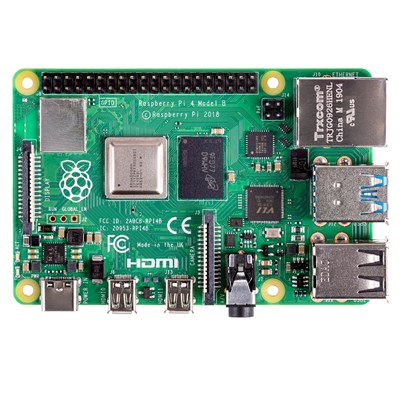
\includegraphics[scale=0.6]{raspberry_pi_4}
\end{center}
The chosen target for this project is the Raspberry Pi 4 Model B, a single board computer developed by 
the Raspberry Pi Foundation and realeased in 2019. The tech specs include:
\begin{itemize} 
    \item Broadcom BCM2711, Quad core Cortex-A72 (ARM v8) 64-bit SoC @ 1.5Ghz
    \item 1GB, 2GB, 4GB, or 8GB LPDDR4-3200 SDRAM (depending on model)
    \item 2.4 GHz and 5.0 Ghz 802.11ac wireless
    \item Gigabit Ethernet
    \item Bluetooth 5.0, BLE
    \item 2 USB 3.0 ports, 2 USB 2.0 ports
    \item Raspberry Pi standard 40 pin GPIO header
    \item 2 micro-HDMI ports (up to 4kp60 supported)
    \item 2-lane MIPI DSI display port
    \item 2-lane MIPI CSI camera port
    \item 4-pole stereo audio and composite video port
    \item H.265 (4kp60 decode), H.264 (1080p60 decode, 1080p30 encode)
    \item OpenGL ES 3.1, Vulkan 1.0
    \item Micro-SD card slot for loading operating system and data storage
    \item 5V DC via USB-C connector (minimum 3A)
    \item 5V DC via GPIO header (minimum 3A)
    \item Power over Ethernet (PoE) enabled (requires separate PoE HAT)
    \item Operating temperature 0 - 50 °C ambient
\end{itemize}

\subsection{FT232-AZ USB to TTL serial UART adapter}

\begin{center}
    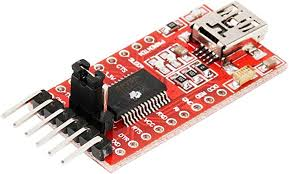
\includegraphics[scale=0.4]{uart_adapter}
\end{center}
The FT232-AZ USB to TTL serial UART adapter is used to connect the PC used during the development of the project
to the target in order to send and receive data between the PC and the Raspberry Pi 4. 
The PC is connected through a USB port, the target is connected through GPIO pins according to the 
following table.

\begin{center}
    \begin{tabular}{ |c|c|c| } 
        \hline
        GPIO & Function & UART adapter  \\
        \hline
        14 (Tx) & Output & Rx \\ 
        15 (Rx) & Input & Tx \\ 
        Ground & Ground & Ground \\ 
        \hline
    \end{tabular}
\end{center}

\subsection{KY-003 Hall sensor}

\begin{center}
    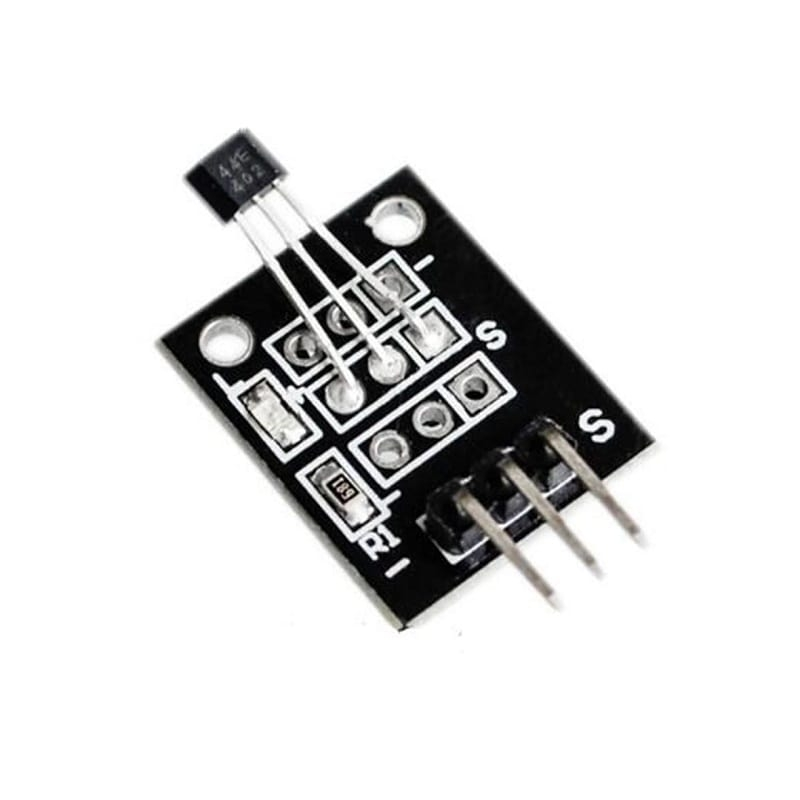
\includegraphics[scale=0.2]{ky-003}
\end{center}
The KY-003 hall sensor allows to detect a magnetic field. When the magnetic field at the Hall sensor exceeds
the operate point threshold (BOP) the output of the device switches low. When the magnetic field is reduced
to below the realease point threshold (BRP) the device output switches high.
BOP and BRP may vary respectively from 1 mT to 33 mT and from 5 mT to 35 mT at operating 
temperature T = 25° C depending on the sensor model.
This sensor is used to trigger the alarm when the magnet is far from the sensor.

\subsection{KY-012 Buzzer}

\begin{center}
    
\includegraphics[scale=0.4]{ky-012}
\end{center}
The KY-012 Buzzer is an active piezoelectric buzzer, it generates a sound of approximately 2.5kHz when 
input signal (S) is high. The Buzzer is activated when the Hall sensor does not detect the magnet.

\subsection{LEDs}

\begin{center}
    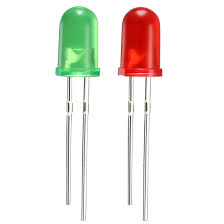
\includegraphics[scale=0.4]{leds}
\end{center}
The LEDs are used to show the alarm status. When the Hall sensor does not detects the magnet the green LED turns off 
and the red LED turns on. When the Hall sensor detect the magnet and the push button is pressed, the green LED turns on
and the red LED turns off.

\subsection{Push Button}

\begin{center}
    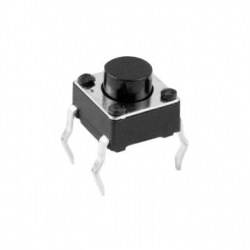
\includegraphics[scale=0.5]{push_button}
\end{center}
The push button can be used to turn off the alarm when the hall sensor detects the magnet.

\subsection{Resistors}

\begin{center}
    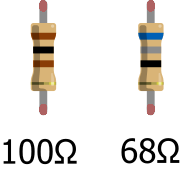
\includegraphics{resistors}
\end{center}
The resistors are connected in series to the LEDs to limit the current flowing through the LED and to ensure that the supplied 
voltage does not exceeds the maximum voltage of the LED. The 100 $ \Omega $ resistor is connected to the red LED, the 68 $ \Omega $ 
resistor is connected to the green LED.

\subsection{LCD 1602}
The LCD 1602 is a liquid crystal display that can display 16x02 characters at the same time. 
This module provides a 16 pin interface and a I2C interface. 
It is used to show the door status (open or closed).

\subsection{PCF8574AT 8-bit I/O expander for I2C bus}

\subsection{GPIO wiring diagram}

\begin{center}
    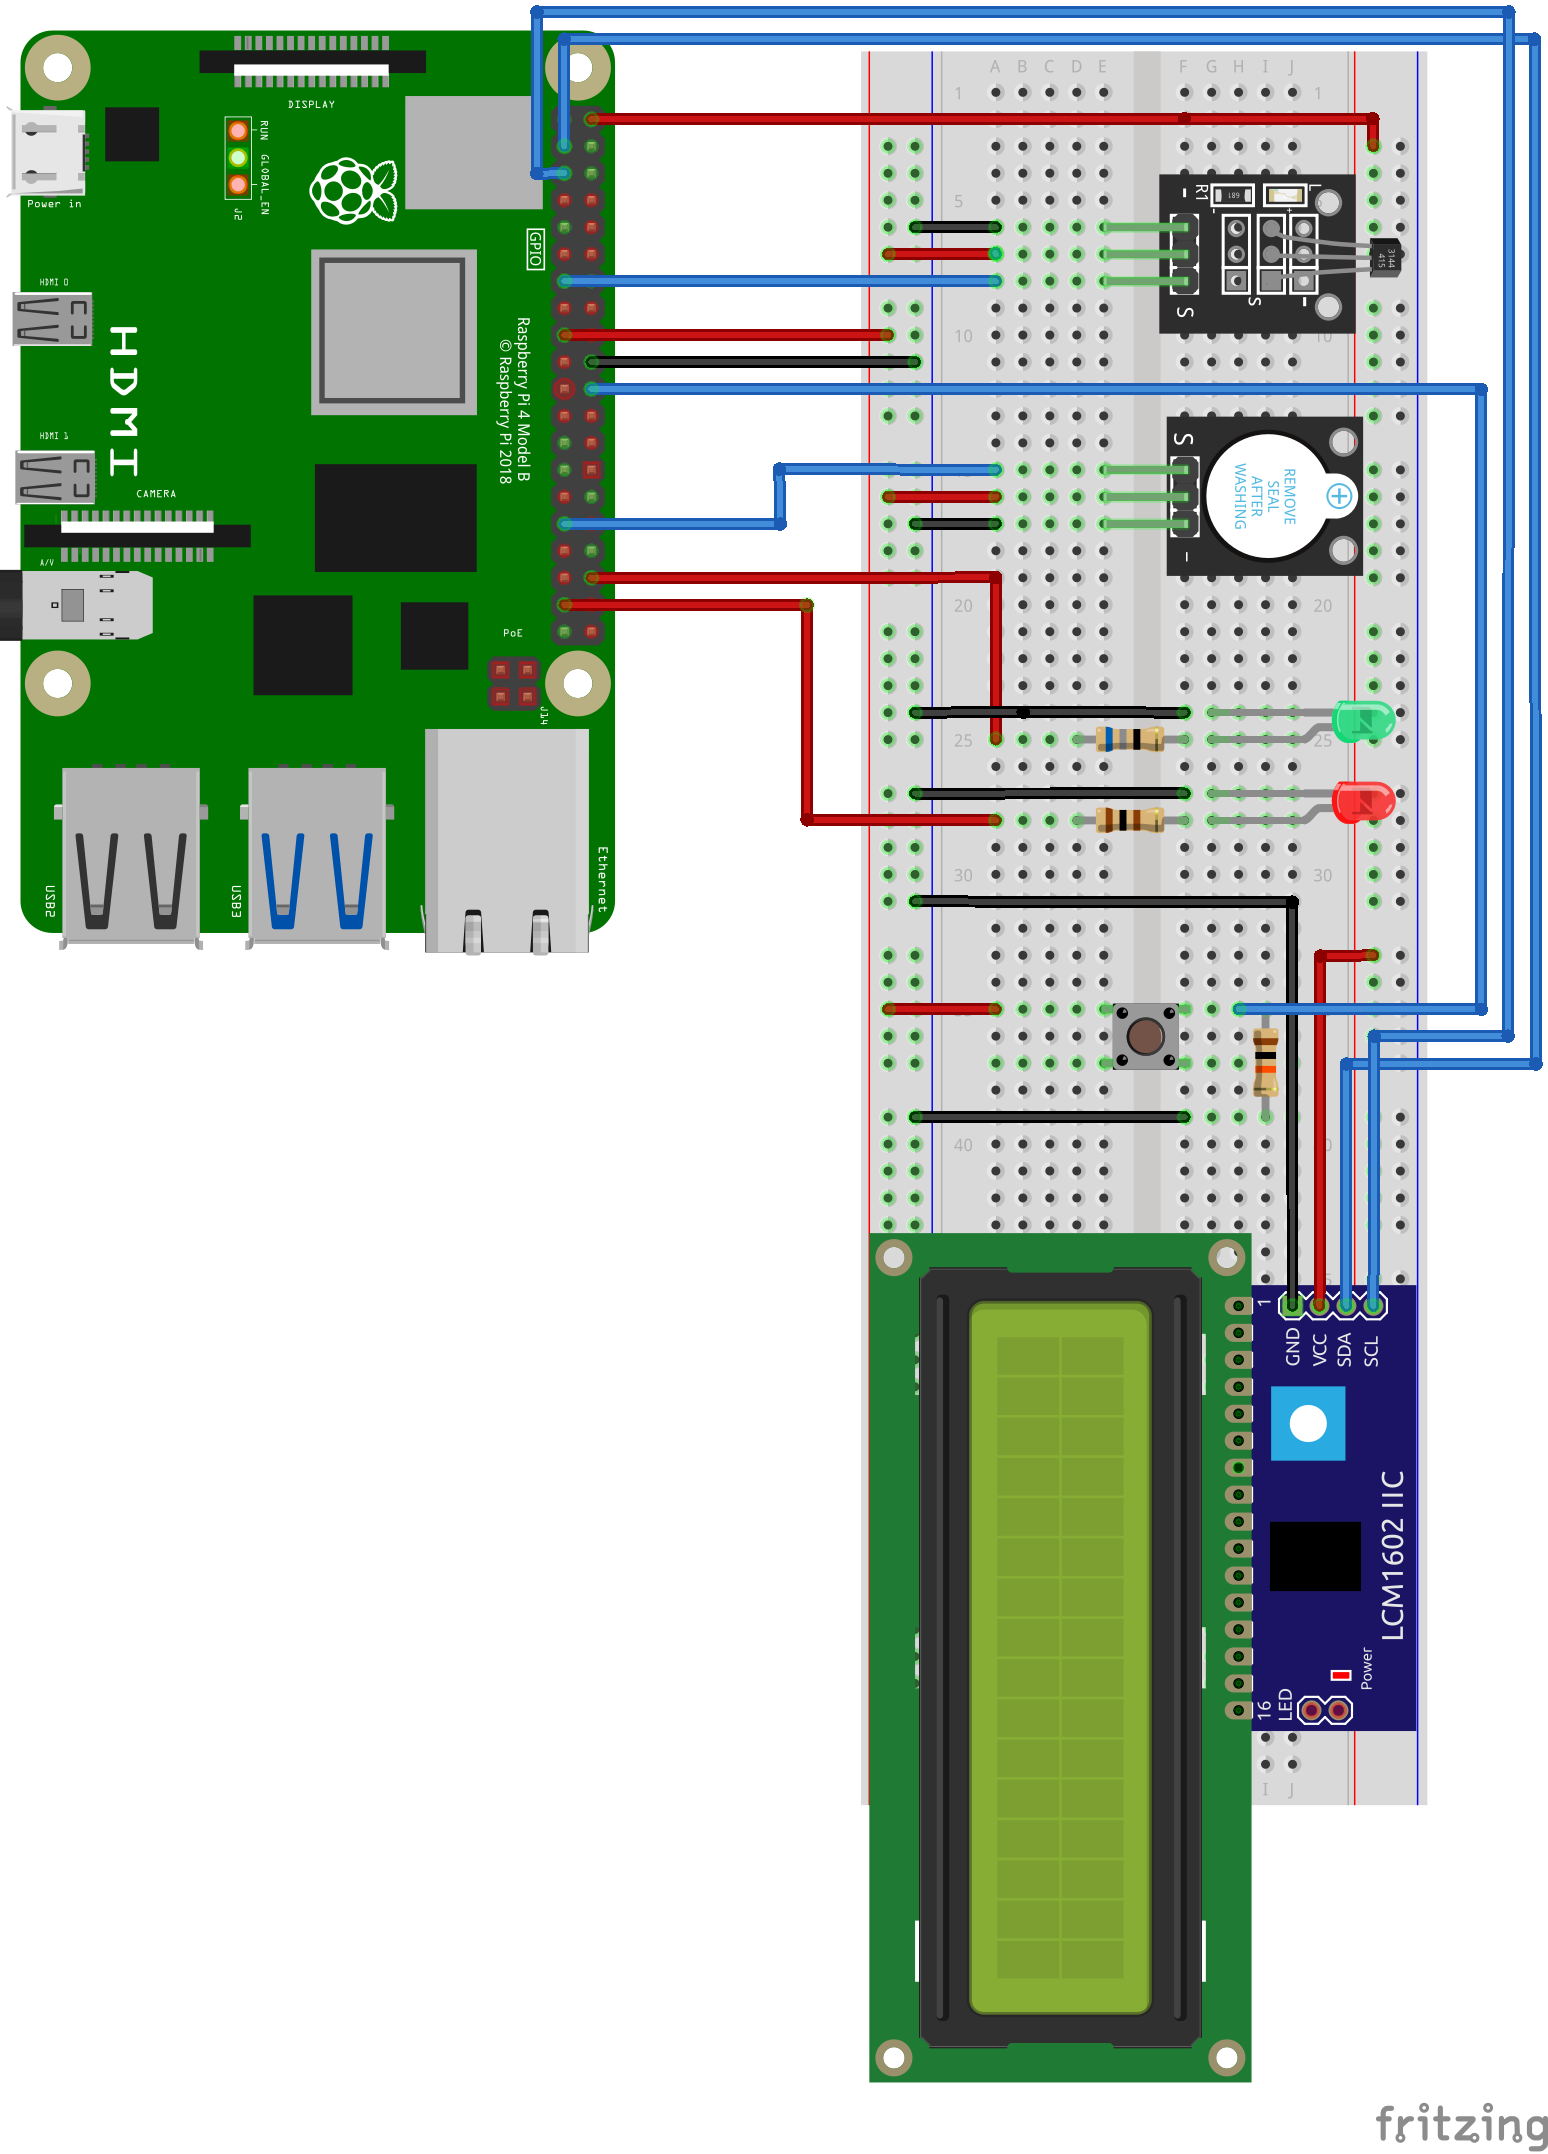
\includegraphics[scale=0.9]{breadboard}
\end{center}

\newpage
The following table is the GPIO wiring diagram.

\begin{center}
    \begin{tabular}{ |c|c|c| } 
        \hline
        GPIO & Function & Connection \\
        \hline
        2 & SDA & SDA (I/O expander) \\
        3 & SCL & SCL (I/O expander) \\
        6 & Output & S (Buzzer) \\
        16 & Output & Anode (Green LED) \\
        25 & Input & Button \\
        26 & Output & Anode (Red LED) \\
        27 & Input & S (Hall sensor) \\
        5V & Power & VCC (I/O expander) \\
        3V3 & Power & Breadboard \\
        Ground & Ground & Breadboard \\
        \hline
    \end{tabular}
\end{center}

\section{Software}

\section{References}

\begin{itemize}
    \item raspberrypi.com/products/raspberry-pi-4-model-b/specifications
    \item cdn.shopify.com/s/files/1/1509/1638/files/FT232-AZ\_Adapter\_Datenblatt\_AZ-Delivery-
    \\\_Vertriebs\_GmbH.pdf
    \item cdn.shopify.com/s/files/1/1509/1638/files/Hall\_Sensor\_Modul\_Digital\_Datenblatt.pdf
    \item cdn.shopify.com/s/files/1/1509/1638/files/KY-012\_Buzzer\_Modul\_Aktiv\_Datenblatt-
    \\\_AZ-Delivery\_Vertriebs\_GmbH.pdf
\end{itemize}



\end{document}